\subsection{Összefoglaló feladatok}


\newcounter{feladatSzamlalo}

%_
\begin{frame}
  Készítse el a \hiv{\href{https://hu.wikipedia.org/wiki/Cascading_Style_Sheets}{CSS wiki oldala}} által ihletett weblapot!
  \begin{columns}[c]
    \column{0.25\textwidth}
      \begin{exampleblock}{\textattachfile{css.html}{css.html}}
        
\includegraphics[width=\textwidth]{css1.pdf}
      \end{exampleblock}
    \column{0.75\textwidth}
      \begin{enumerate}
        \scriptsize
        \item Induljon ki a \textattachfile{css.txt}{css.txt} fájlból!
        \item Készítsen ebből magyar nyelvű HTML5 dokumentumot, UTF-8 karakterkódolással!
        \item Az oldal első szintű címsora és a böngészőfülön megjelenő szöveg egyaránt legyen ,,Cascading Style Sheets''!
        \item Ezt válassza el egy vízszintes vonallal...
        \item ...a második szintű címsorként jelölt sortól (,,A Wikipédiából, \dots'')! A ,,Tartalomjegyzék'' és az ,,Áttekintés'' szintén 2. szintű címsorként legyen jelölve!
        \item Az első bekezdés elején álló ,,CSS''-t jelölje meg rövidítésként! Ha valaki fölötte tartja az egeret, jelenjen meg a ,,Cascading Style Sheets, magyarul: lépcsőzetes stíluslapok'' szöveg egy buborékban!
        \item Jelölje meg hivatkozásként a ,,HTML'' szót, ami a megfelelő Wikipédia oldalra mutat!
        \item Járjon el ugyanígy az ,,XHTML''-lel is, de azt új fülön nyissa meg!
        \setcounter{feladatSzamlalo}{\theenumi}
      \end{enumerate}
  \end{columns}
\end{frame}

%_
\begin{frame}
  \begin{columns}[c]
    \column{0.25\textwidth}
      \begin{exampleblock}{\textattachfile{css.html}{css.html}}
        
\includegraphics[width=\textwidth]{css2.pdf}
      \end{exampleblock}
    \column{0.75\textwidth}
      \begin{enumerate}
        \footnotesize
        \setcounter{enumi}{\thefeladatSzamlalo}
        \item A dokumentum tartalma alkosson egy cikket!
        \item Minden, ami a tartalomjegyzék felett van, legyen fejlécként jelölve!
        \item Külön szakaszként jelölje a tartalomjegyzéket, és az azt követő fő fejezeteket (,,Áttekintés'', ,,A CSS használata'')!
        \item A tartalomjegyzék pontjait egymásba ágyazott, számozott listák alkossák!
        \item Ezek egyúttal legyenek hivatkozások a dokumentumon belüli fejezetekre!
        \item Az ,,Áttekintés'' fejezetben hozzon létre nem számozott felsorolást!
        \item A kötőjel előtti részt jelölje meg hangsúlyos szövegrészként!
        \item A kötőjeleket cserélje közepes hosszúságú gondolatjelekre!
        \item A felsorolás pontjaiban szereplő *-ot, HTML elemneveket, stb. jelölje meg programkódként!
        \setcounter{feladatSzamlalo}{\theenumi}
      \end{enumerate}
  \end{columns}
\end{frame}

%_
\begin{frame}
  \begin{columns}[c]
    \column{0.25\textwidth}
      \begin{exampleblock}{\textattachfile{css.html}{css.html}}
        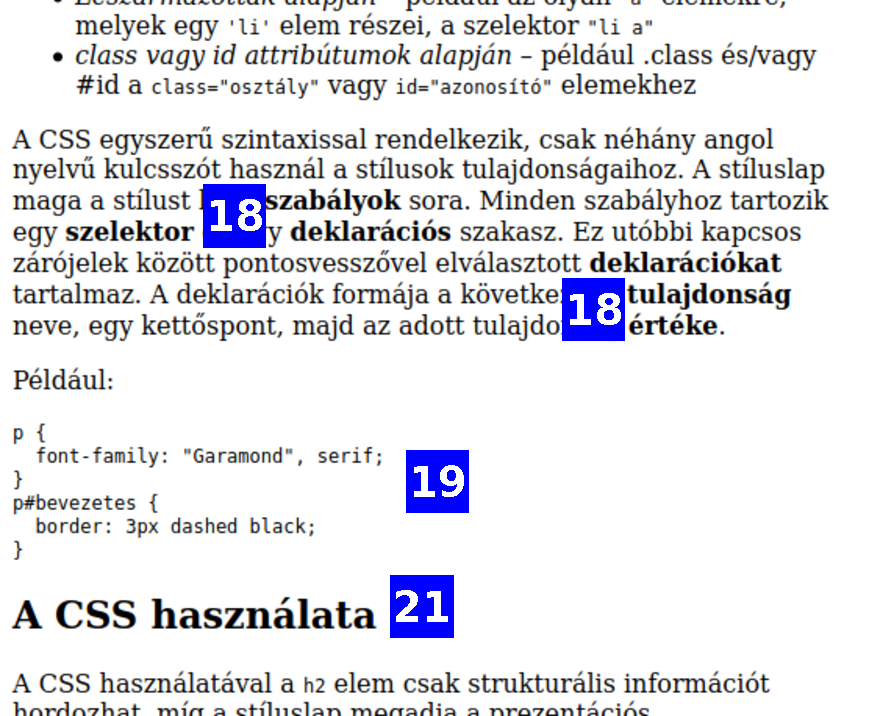
\includegraphics[width=\textwidth]{css3.pdf}
      \end{exampleblock}
    \column{0.75\textwidth}
      \begin{enumerate}
        \setcounter{enumi}{\thefeladatSzamlalo}
        \item A felsorolást követő szövegben a fontos fogalmakat (szabályok, szelektor, deklarációs, \dots) jelölje meg félkövérrel szedendő szövegként!
        \item A példaként szereplő CSS szöveget jelölje meg előformázott szövegrésznek!
        \item A CSS kód töredékeit ágyazza be olyan, előredefiniált jelentéssel nem bíró soron belüli elembe, melynek \texttt{class} attribútuma utal a kód azon részének szemantikai töltetére, pl. a \texttt{p} elemnévnél az attribútum értéke lehet \texttt{element}, a \texttt{bevezetes}-nél \texttt{id}, a \texttt{font-family} tulajdonságnál \texttt{property}, a kettőspont utáni részeknél \texttt{value}, stb.!
        \item Jelölje meg 2. szintű címsorként ,,A CSS használata'' sort!
        \setcounter{feladatSzamlalo}{\theenumi}
      \end{enumerate}
  \end{columns}
\end{frame}
